\section{Shape reconstruction}
\label{sec:recon}

Reconstructing geometric shapes from physical objects is a fundamental problem in geometry processing. \rev{The input to this problem is usually a point cloud produced by aligned range scans, which provides an observation of an object. The goal of a shape reconstruction algorithm is to convert this point cloud into a high-quality geometric model. In practice, the input point cloud data is noisy and incomplete. Thus, the key to a successful shape reconstruction algorithm is formulating appropriate shape priors. \rev{Traditional shape reconstruction algorithms usually utilize generic priors, such as surface smoothness \cite{Diebel:2005:BMP}, and typically assume that the input data captures most of the object's surface.} To handle higher degrees of noise and partiality of the input data, it is important to build structural shape priors.}
%They tend to fail when the input point cloud is produced by consumer-level depth cameras, where the resulting scans usually exhibit high degree of noise. In this case, we need more global and structural shape priors for obtaining high quality geometry reconstruction.

\rev{Data-driven techniques tackle this challenge by leveraging shape collections to learn strong structural priors from similar objects, and use them to reconstruct high-quality 3D models. Existing approaches fall into two categories, based on how they represent the shape priors: \textsl{parametric} and \textsl{non-parametric}. The former usually builds a low-dimensional parametric representation of the underlying shape space, learning the representation from exemplars and enforcing the parameterization when reconstructing new models. Parametric methods typically require building correspondences across the exemplar shapes.
%, and thus they are mostly suitable for organic shapes or shapes with small variation, such as human bodies and faces. \vangelis{this is a strong statement - i do not agree with this. Parameters can include point and part existences, which means that can handle variations}
In contrast, non-parametric methods directly operate on the input shapes by copying and deforming existing shapes or shape parts.}
%On the other hand, their performance relies on effective and efficient tools for both shape retrieval and deforming/assembling retrieved shapes.

\subsection{Parametric methods}

\begin{figure}[t]
\centering
    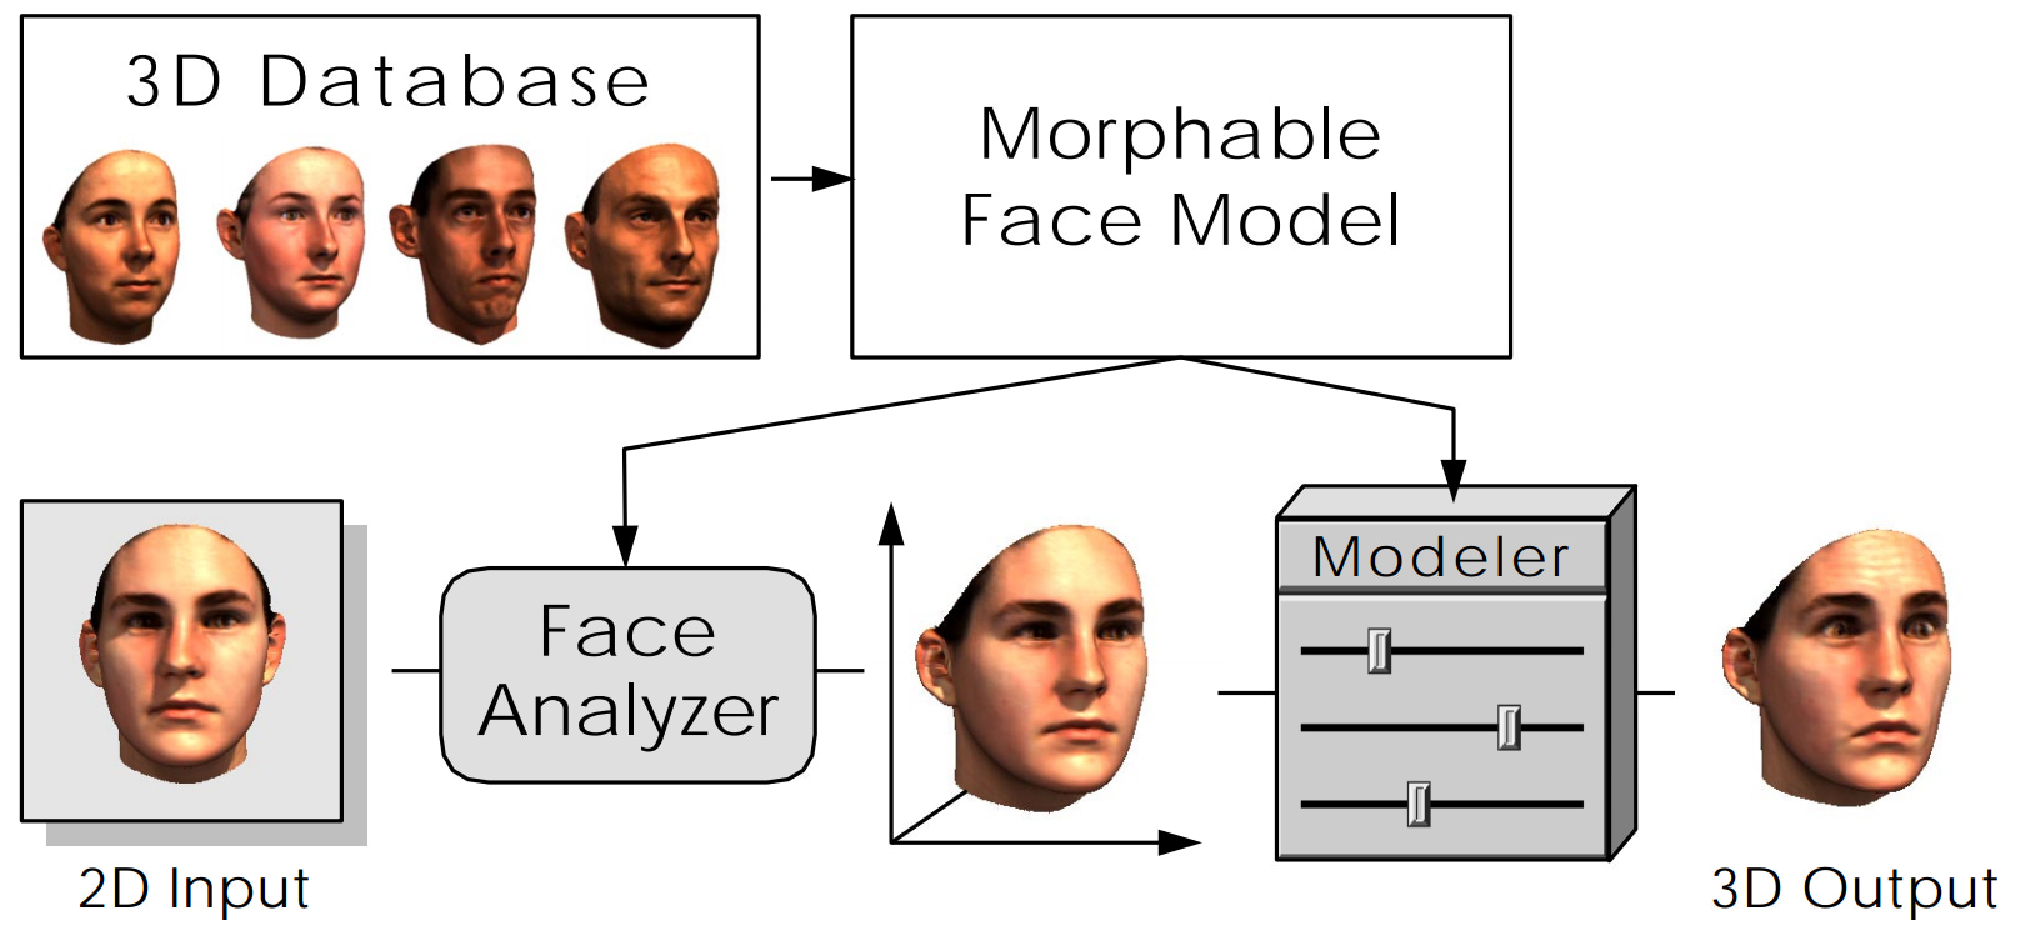
\includegraphics[width=1.0\columnwidth]{fig/img/blanz_sig99_face.pdf}
    %\vspace{-0.4cm}
    \caption{Derived from a dataset of prototypical 3D scans of faces, the morphable face model contributes to two main steps in face manipulation: (1) deriving a 3D face model from a novel image, and (2) modifying shape and texture in a natural way~\cite{Blanz:1999:MMS}.}
    \label{fig:blanz_sig99_face}
\end{figure}



\paragraph*{Morphable face.} The morphable face model~\cite{Blanz:1999:MMS} is a representative work of parametric data-driven shape reconstruction,
%Other parametric methods can be described as variants and extensions to this method.
a technique which reconstructs 3D textured faces from photos and scans. The model is learned from a dataset of prototypical 3D shapes of faces, and can then be used to derive a new 3D face from a novel image. (See Figure\ref{fig:blanz_sig99_face}).

In particular, the morphable face model represents the geometry of a face with a shape-vector $S = (\mathbf{p}_1^{T}, \cdots, \mathbf{p}_{n}^{T})^{T}) \in \mathbb{R}^{3n})$, that contains the 3D coordinates of its $n$ vertices. Similarly, it encodes the texture of a face by a texture-vector $T = (\vec{c}_1^{T}, \vec{c}_2^{T}, \cdots, \vec{c}_{n}^{T}) \in \mathbb{R}^{3n}$, that contains the RGB color values of the corresponding vertices. A morphable face model is then constructed using a database of $m$ exemplar faces, each represented by its shape-vector $S_i$ and $T_i$. In~\cite{Blanz:1999:MMS} the exemplar faces are constructed by matching a template to scanned human faces.

%Given these exemplar faces, new shapes $S_{\textup{mod}}$ and new textures $T_{\textup{mod}}$ c%an be expressed in barycentric coordinates as a linear combination of the shapes and textures:
%$$
%\vec{S}_{\textup{mod}} = \sum\limits_{i=1}^{m}a_i\vec{S}_{i} , \quad T_{\textup{mod}} = \sum\limits_{i=1}^{m}b_i\vec{T}_{i}, \quad \sum\limits_{i=1}^{m}a_i = \sum\limits_{i=1}^{m}b_i = 1.
%$$
%In other words, a morhpable model is given by the set of faces $(\vec{S}_{\textup{mod}}(\vec{a}), T_{\textup{mod}}(\vec{b}))$, parameterized by the coefficients $\vec{a} = (a_1, \cdots, %a_{m})^{T}$ and $\vec{b} = (b_1, \cdots, b_{m})^{T}$. Arbitrary new faces can be generated by varying the parameters $\vec{a}$ and $\vec{b}$ that control shape and texture.

%In addition to learning a generative model, it is important to quantify the likelihood of different regions in the parameter space. Blanz et al.~\cite{Blanz:1999:MMS} use example faces to estimate the probability distribution for the coefficients $\vec{a}$ and $\vec{b}$, which quantifies the plausibility of faces sampled from the generative model. They use
%
%Another data-driven perspective of the morphable face model is to quantify the results in terms of their plausibility of being faces. As describe in~\cite{Blanz:1999:MMS}, one way is to estimate the probability distribution for the coefficients $\vec{a}$ and $\vec{b}$ from the example faces. This distribution enables us to control the likelihood of the coefficients $\vec{a}$ and $\vec{b}$ and consequently regulate the likelihood of the appearance of the generated faces. The specific technique employed by~\cite{Blanz:1999:MMS} is
The morphable face model uses Principal Component Analysis (PCA) to characterize the shape space. A new shape and its associated texture are given by
%, which performs a basis transformation to an orthogonal coordinate system formed by the eigenvectors $\vec{s}_i$ and $\vec{t}_i$ of the covariance matrices:
$$
\vec{S}_{\textup{mod}} = \overline{\vec{S}} + \sum\limits_{i=1}^{m-1}\alpha_i \vec{s}_i, \quad \vec{T}_{\textup{mod}} = \overline{\vec{T}} + \sum\limits_{i=1}^{m-1}\beta_i \vec{t}_i,
$$
where $\overline{\vec{S}}$ and $\overline{\vec{T}}$ are the mean-shape and mean-texture, respectively, and $\vec{s}_i$ and $\vec{t}_i$ are eigenvectors of the covariance matrices. $\alpha_i$ and $\beta_i$ are coefficients. PCA also gives probability distributions over coefficients. The probability for coefficient $\alpha_i$ is given by
$$
p(\{\alpha_i\}) \sim \exp\left(-\frac{1}{2}\sum\limits_{i=1}^{m-1}(\alpha_i/\sigma_i)^2\right),
$$
with $\sigma_i^2$ being the corresponding eigenvalue of the shape covariant matrix $C_{S}$ (the probability $p(\{\beta_i\})$ is computed in a similar way).

With this morphable face model, reconstruction of textured models can be posed as a small-scale non-linear optimization problem. For example, given a 2D image of a human face $I_{\textup{input}}$, one can reconstruct the underlying textured 3D model by searching for a similar rendered face $I(\{\alpha_i\},\{\beta_i\}, p)$, parameterized by the shape and texture coefficients $\alpha_i$ and $\beta_i$, and the rendering parameters $p$ (e.g., camera configuration, lighting parameters). The optimization problem is formulated as minimizing a data term, which measures the distance between the input image and the rendered image, and regularization terms that are learned from exemplar faces. The success of the morphable model relies on the low-dimensionality of the solution space, and so is also applicable to several other data sets where this assumption holds, including the domain of human bodies and poses.

%The success of the morphable model relies on the low-dimensionality of the optimization problem, as well as the regularization terms that control the behavior of the objective function.
%Both properties are enabled have exemplar models. In the following, we discuss several other representative parametric data-driven shape reconstruction methods.

\begin{figure}[t]
\centering
    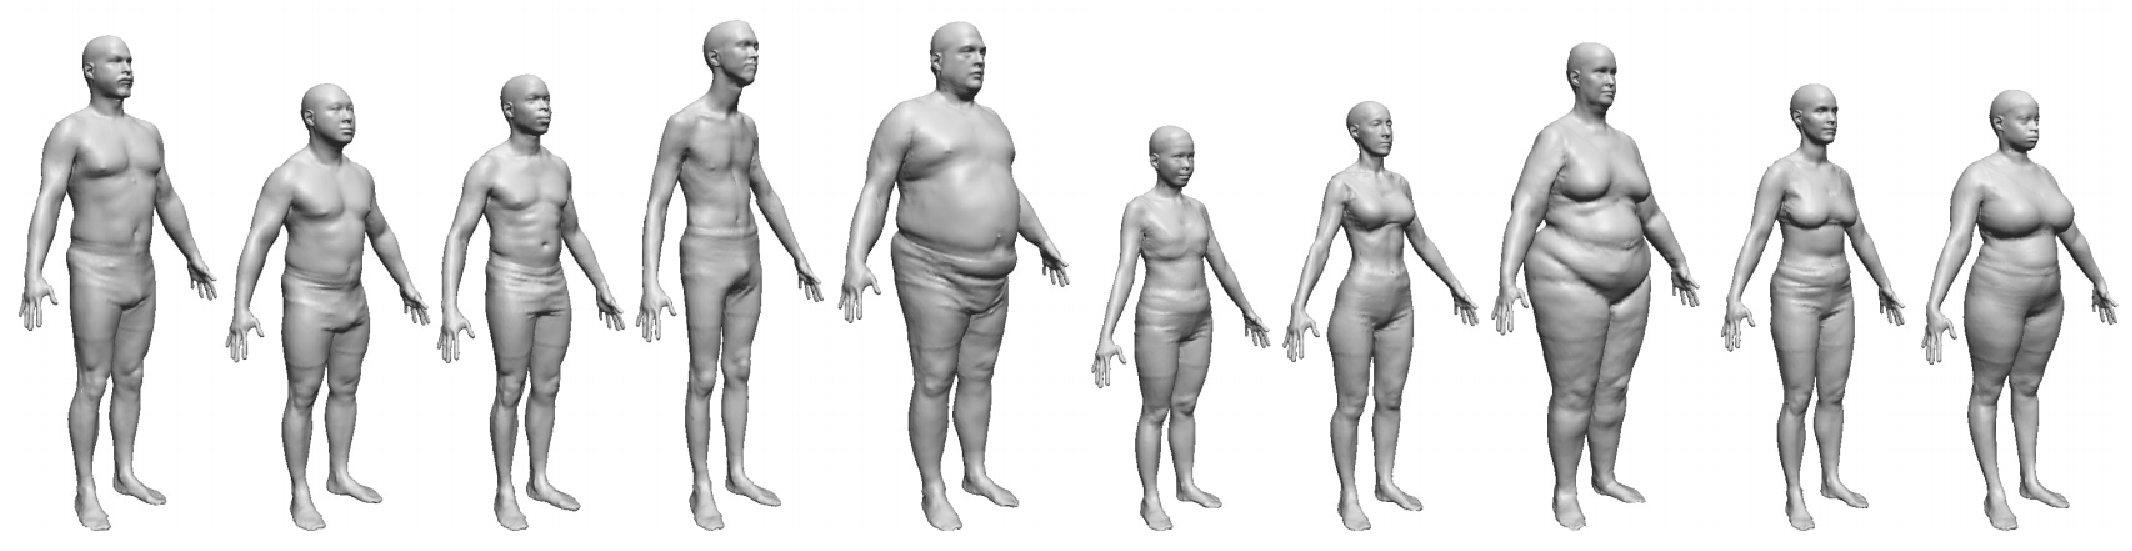
\includegraphics[width=1.0\columnwidth]{fig/img/allen_sig03_human.pdf}
    %\vspace{-0.4cm}
    \caption{Parameterizing the variation in human shapes can be used to synthesize new individuals or edit existing ones~\cite{Allen:2003:SHB}.}
    \label{fig:allen_sig03_human}
\end{figure}



\paragraph*{Morphable human bodies.} \rev{Allen et al.~\cite{Allen:2003:SHB} generalize the morphable model to characterize human bodies (Figure ~\ref{fig:allen_sig03_human}). Given a set of $250$ scanned human bodies, the method first performs non-rigid registration to fit a hole-free, artist-generated mesh (template) to each of these scans. The result is a set of mutually consistent parameterized shapes based on the corresponding vertex positions originating from the template. Similar to~\cite{Blanz:1999:MMS}, the method employs PCA to characterize the shape space, which enables applications in shape exploration, synthesis and reconstruction.}

In addition to variations in body shape, human models also exhibit variations in poses.  The SCAPE model (Shape Completion and Animation for People)~\cite{SCAPE:2005} addresses this challenge by learning two separate models of body deformation -- one accounting for variations in poses and one for differences in body shapes. The pose deformation component is acquired from a set of dense 3D scans of a single person in multiple poses. A key aspect of the pose model is that it decomposes deformation into a rigid and a non-rigid component. The rigid component is modeled using a standard skeleton system. The non-rigid component, which captures remaining deformations such as flexing of the muscles, associates each triangle with a local affine transformation matrix. These transformation matrices are learned from exemplars using a joint regression model. %Similar to previous works, SCAPE models body variations using PCA from different people in different poses.
%
In~\cite{Hasler:2009:SSR}, Hasler et al. introduce a unified model for parameterizing both shapes and poses. The basic idea is to consider the relative transformations between all pairs of neighboring triangles. These transformation matrices allow us to reconstruct the original shape by solving a least squares problem. In this regard, each shape is encoded as a set of edge-wise transformation matrices, which are fit into the PCA framework to obtain a statistical model of human shapes. The model is further extended to estimate shapes of dressed humans from range scans~\cite{Hasler:2009:TSE}.

\rev{Recent works on statistical human shape analysis focus on combining learned shape priors with sparse observations and special effects. In~\cite{Loper:SIGASIA:2014}, the authors introduce an approach that reconstructs high-quality shapes and poses from a sparse set of markers. The success of this approach relies on learning meaningful shape priors from a database consisting of thousands of shapes. In~\cite{Tsoli:2014:BLS}, the authors study human breathing from acquired data.}

% statistical human models
%\cite{}Bogo:CVPR:2014 Freifeld:2012:LBM
%\begin{figure}[t]
\centering
    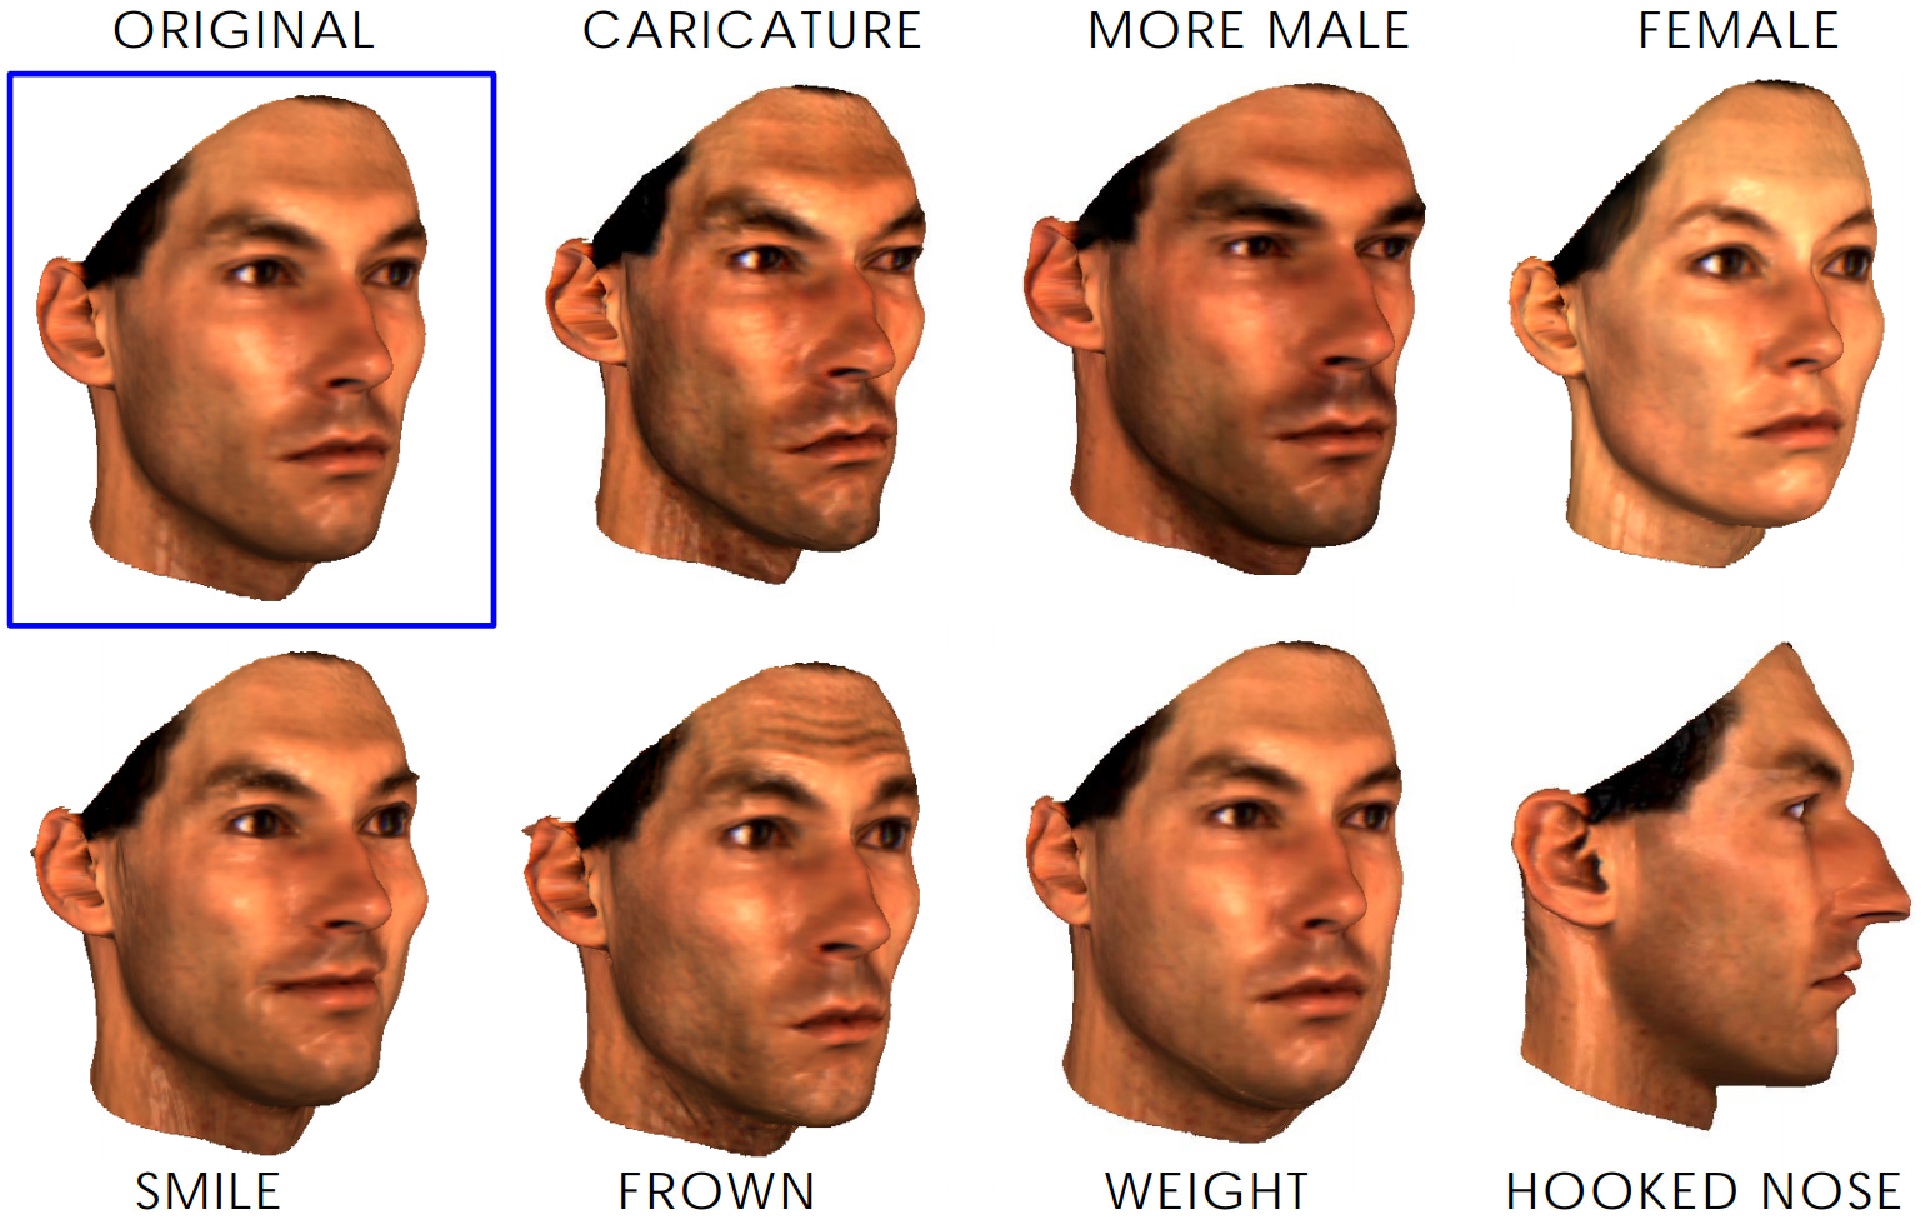
\includegraphics[width=1.0\columnwidth]{fig/img/blanz_sig99_attris.pdf}
    \vspace{-0.4cm}
    \caption{Variation of facial attributes of a single face. The appearance of the original face can be changed by adding and subtracting shape and texture vectors specific to the attribute.}
    \vspace{-0.6cm}
    \label{fig:blanz_sig99_attris}
\end{figure}


%\para{Learning shape attributes.} Besides shape reconstruction, the learned parametric shape space models can also be applied to learn shape attributes, such as facial expressions and semantic human body attributes. The morphable face model~\cite{Blanz:1999:MMS} learns facial attributes as linear combinations of positional displacements between the exemplar faces and the mean face. \cite{Li:2010:EFR} applies a similar model for face rigging.

%For human shapes existing methods~\cite{Allen:2003:SHB,SCAPE:2005,Hasler:2009:SSR} learn human body attributes such as height, weight, body fat, waist girth. Similar to faces, these attributes are described as vectors (with respect to the mean space) in the parametric shape spaces. Recently, \cite{Zhou:2010:PRH} applies these shape attributes to applications in parametric reshaping of human bodies.


\paragraph*{Data-driven tracking.} Object tracking aims to analyze dynamic shapes and/or poses of physical objects. Successful tracking techniques (e.g.,~\cite{Weise:2009:FLF,Weise:2011:RPF,Li:2013:RFA,Cao:2013:SRR,Cao:2014:DDE}) typically utilize parametric shape spaces. These reduced shape spaces provide shape priors that improve both the efficiency and robustness of the tracking process. The way to utilize and construct shape spaces vary in different settings, and are typically tailored to the specific problem setting. Weise et al.~\cite{Weise:2009:FLF} utilize a linear PCA subspace trained with a very large set of pre-processed facial expressions. This method requires an extended training session with a careful choice of facial action units. In addition, the learned face model is actor-specific. These restrictions are partially resolved in~\cite{Li:2010:EFR}, which introduces an example-based blendshape optimization technique, involving only a limited number of random facial expressions.
In~\cite{Weise:2011:RPF}, the authors combine both blendshapes and data-driven animation priors to improve the tracking performance. In a recent work, Li et al.~\cite{Li:2013:RFA} employ adaptive PCA to further improve tracking performance on nuanced emotions and micro-expression. The key idea is to combine a general blendshape PCA model and a corrective PCA model that is updated on-the-fly. This corrective PCA model captures the details of the specific actor and missing deformations from the initial blendshape model.

\vspace{-.2cm}

\subsection{Non-parametric methods}

\rev{Parametric methods require canonical domains to characterize the shape space, which have so far been demonstrated within domains of organic shapes,  such as body shapes or faces.
%, where such a canonical domain can be easily built.
%Thus, they are suitable for organic shapes such as body shapes or faces, where such a canonical domain exists. They become less effective on shapes that undergo significant geometrical and topological variations (e.g., man-made objects). \vangelis{strong statement - i do not agree that this is entirely true}
In this section, we discuss another category of methods that have shown the potential to handle more diverse shape collections.}

Generally speaking, a non-parametric data-driven shape reconstruction method utilizes a collection of relevant shapes and combines three phases, i.e., a query phase, a transformation phase and an assembly phase. Existing methods differ in how the input shape collection is preprocessed and how these phases are performed.

\begin{figure}[t]
\centering
    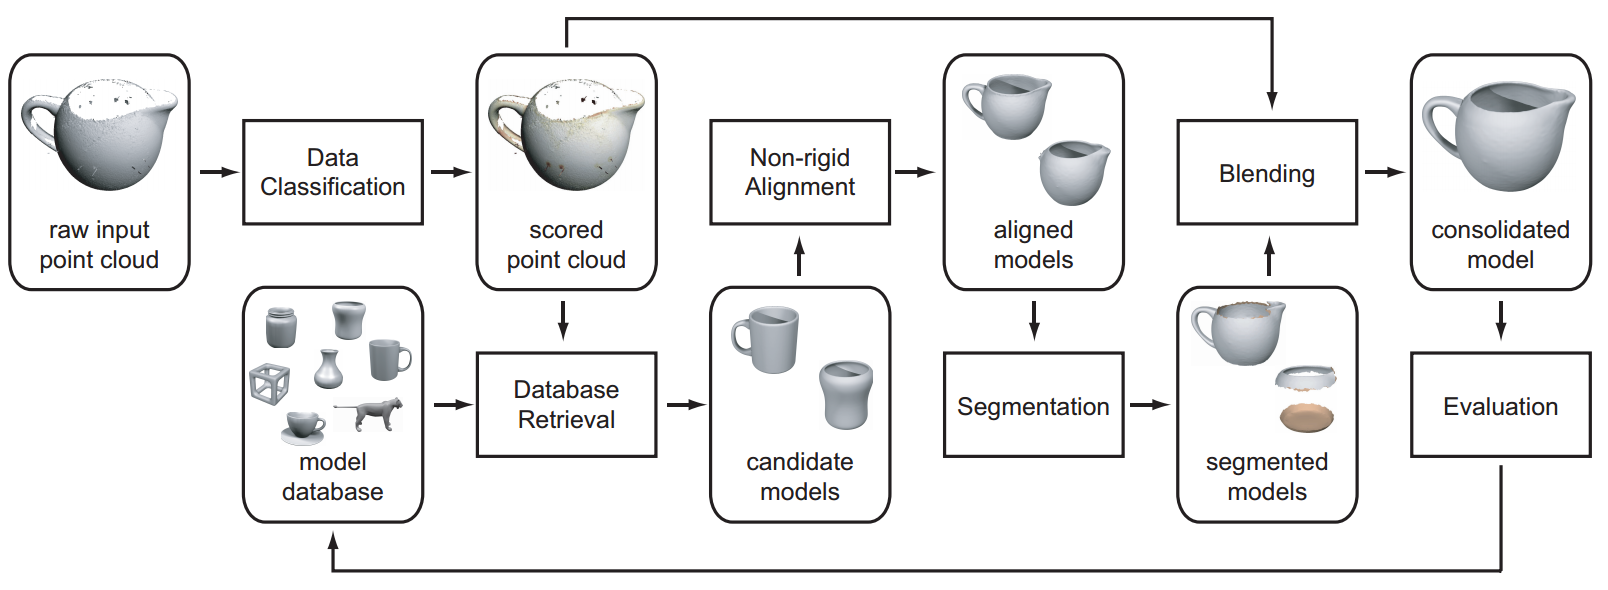
\includegraphics[width=1.0\columnwidth]{fig/img/pauly_sgp05_esr.png}
    %\vspace{-0.5cm}
    \caption{The data-driven shape reconstruction pipeline proposed in~\cite{Pauly:2005:ESC}.}
    \label{fig:pauly_sgp05_esr}
\end{figure}


\paragraph*{Example-based scan completion.} Pauly et al.~\cite{Pauly:2005:ESC} introduce one of the first non-parametric systems. As shown in~\cite{Pauly:2005:ESC}, the method takes a point cloud and a collection of complete objects as input. The reconstruction procedure incorporates all three phases described above. The first phase determines a set of similar objects. The retrieval phase combines both text-based search and PCA signatures, which are then refined by rigid alignment. The second step performs non-rigid alignment between the retrieved shapes and the input point cloud. This step partitions the input point cloud into a set of patches, where each patch is associated with one retrieved shape (via the corresponding region). The final phase merges the corresponding regions into a unified shape.

Nan et al.~\cite{Nan:2012:SAC} introduce a similar system for indoor scene reconstruction. Given an input point cloud of an indoor scene that consists of a set of objects with known categories, the method searches in a database of 3D models to find matched objects and then deforms them in a non-rigid manner to fit the input point cloud. Note that this method treats complete 3D objects as building blocks, so the final reconstruction does not necessarily reflect the original scene.
Shao et al.~\cite{Shao:2012:IAS} adopt an interactive approach to labeled segmentations of RGBD images, followed by 3D model retrieval for scene modeling. Chen et al.~\cite{Chen:2014:ASM} learn contextual relationships from a 3D scene database to further constrain the reconstruction for semantic compatibility between both objects and parts.

In contrast to considering entire 3D shapes, Gal et al.~\cite{Gal:2007:SRU} utilize a dictionary of local shape priors (defined as patches) for shape reconstruction. The method is mainly designed for enhancing shape features, where each region of an input point cloud is matched to a shape patch in the database. The matched shape patch is then used to enhance and rectify the local region. Recently, Mattausch et al.~\cite{MATTAUSCH:2014:ODC} introduce a patch-based reconstruction system for indoor scenes. Their method considers recognizing and fitting planar patches from point cloud data.

Shen et al.~\cite{Shen:2012:SRP} extends this idea for single object reconstruction by assembling object parts. Their method utilizes a collection consistently segmented 3D shapes. Given a scan of an object, the method recursively searches for parts in the collection to assemble the original object. The retrieval phase considers both the geometric similarity between the input and retrieved parts as well as part compatibility which is learned from the input shapes.
\fix{Sung et al.~\cite{Sung15} describe a framework for reliably estimating the part structure of partial scans by treating each part as a local coordinate system.
Their method also utilizes symmetric properties of the target object and shape collection, providing more accurate reconstructions on their shape completion benchmark.}


\begin{figure*}[t]
\centering
    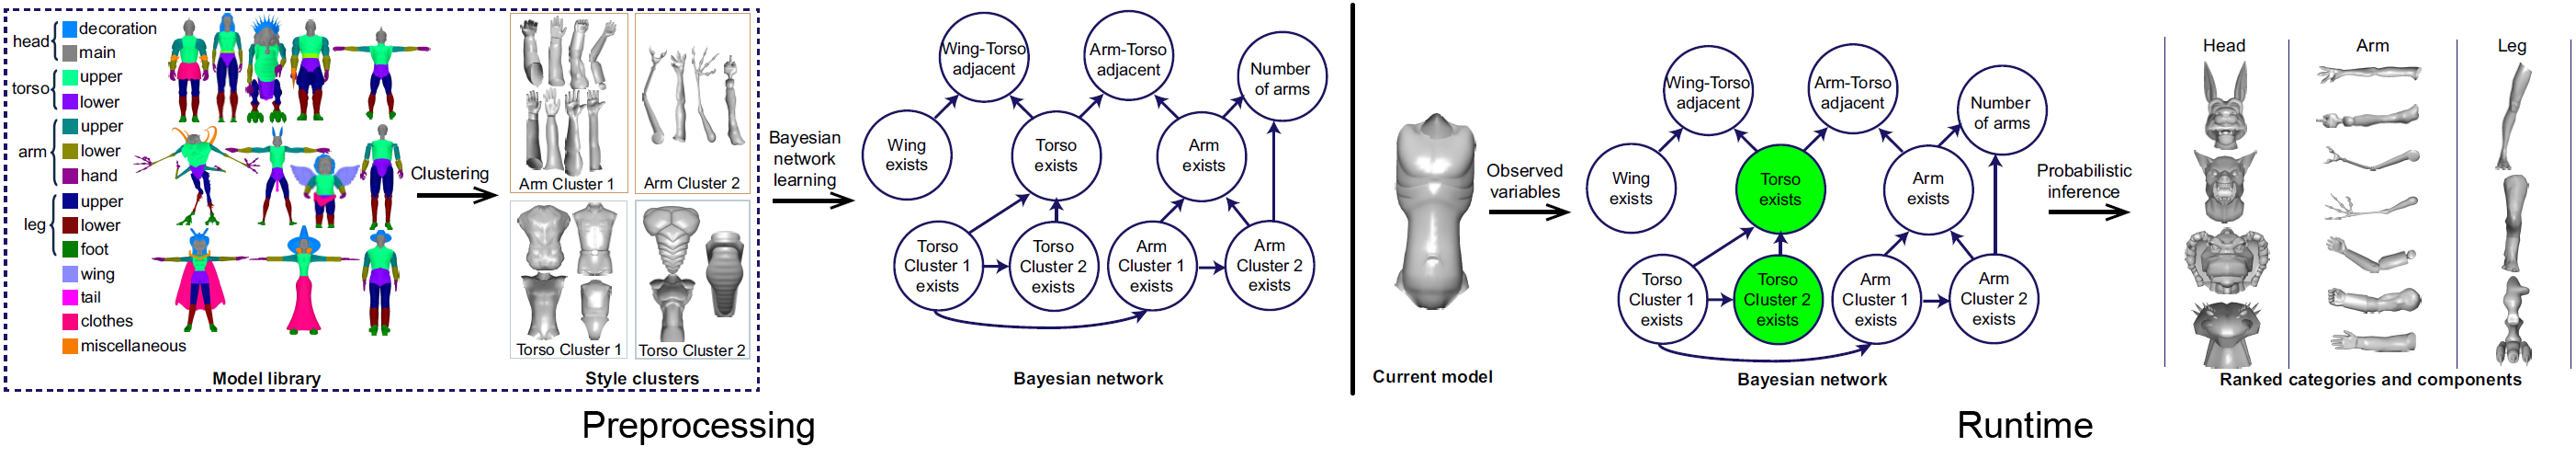
\includegraphics[width=1.0\linewidth]{fig/img/chaudhuri_sig11_prob.png}
    %\vspace{-0.4cm}
    \caption{
    Given a library of models, a Bayesian network encoding semantic and geometric relationships among shape parts
    is learned~\protect\cite{Chaudhuri:2011:prabm} (top). The modeling process (bottom) performs probabilistic inference in the learned
    Bayesian network to generate ranked lists of category labels and components within each category, customized for the currently assembled model.}
    \label{fig:segmentation_labeling}
\end{figure*}



\paragraph*{Data-driven SLAM.} Non-parametric methods have also found applications in reconstructing temporal geometric data (e.g., the output of the Kinect scanner). The Simultaneous localization and mapping (or SLAM) method is a notable technique which jointly estimates the trajectory of the scanning device along side the geometry of the environment. In this case, shape collections serve as priors for the objects in the environment, which can be used to train object detectors. For example, the SLAM++ system proposed by Salas-Moreno et al.~\cite{Salas-Moreno:2013:SLAM} trained domain specific object detectors from shape collections. The learned detectors are integrated inside the SLAM framework to recognize and track those objects. Similarly, Kim et al.~\cite{Kim:2012:AIE} use learned object models to reconstruct dense 3D models from a single scan of an indoor scene. More recently, Sun et al.~\cite{Sun:2014:SS} introduced a 3D sliding window object detector with improved performance and capability extending to a broader range of objects.
\fix{Li et al.~\cite{Li:2015:DA} propose a data-assisted online reconstruction technique which allows object retrieval from a 3D shape database while simultaneously scanning an environment in real-time.}

\paragraph*{Shape-driven reconstruction from images.} Recently, there is a growing interest in reconstructing 3D objects directly from images (e.g.,~\cite{Xu:2011:PMO,Kholgade:2014:OMS,Aubry14,Su:2014:EID}). This problem introduces fundamental challenges in both querying similar objects and deforming objects/parts to fit the input object. In terms of searching similar objects, successful methods typically render objects in the database from a dense set of viewpoints and pick objects where one view is similar to the input image object. Since depth information is missing from the image object, it is important to properly regularize 3D object transformations; otherwise, a 3D object may be deformed arbitrarily even though its projection on the image domain matches the image object. Most existing techniques consider rigid transformations or user-specified deformations~\cite{Xu:2011:PMO}. In a recent work, Su et al.~\cite{Su:2014:EID} propose to learn meaningful deformations of each shape from its optimal deformation to similar shapes.
\fix{Huang et al.~\cite{Huang:SVR:2015} jointly analyze a large collection of images in object categories and a smaller collection of 3D models
to achieve simultaneous analysis and reconstruction of 2D images.}

%\subsection{Discussion and Future directions}

%Despite the progress made in data-driven shape reconstruction, this problem is far-from being solved. The key challenge in parametric methods is to obtain consistently correspondences across the shapes. Existing techniques typically utilize template matching and require a significant amount of manual interaction, which limit them to small-scale datasets (e.g., hundreds of shapes). With the availability large geometric data, it is necessary to scale-up the learning phase of parametric methods, since learning from large shape data would result in more accurate statistics and thus provide better priors for reconstruction. Another challenge of parametric methods is to constrain the shape space so that it avoids infeasible shapes. This is the fundamental limitation of linear shape space methods. One way to address this issue is to perform sampling of feasible shapes (c.f.,~\cite{Wang:2009:RHC}). While it is demanding to develop to alternative ways to characterize shape spaces.

%For non-parametric methods, there is a fundamental tradeoff between the efficiency of shape retrieval and having a large shape collection so that one can always find similar shapes for the object of consideration. Just as what have been done images, developing effective tools that index through 3D shapes plays a central role here. In addition, in many cases the retrieval object/part is similar in global shape but differ in local details to the underlying object. Thus, another challenge of non-parametric methods is how to recover shape details of the underlying object. Note that this problem cannot be resolved by simply deforming the retrieval objects.

%It would be very interesting to extend parametric methods to man-made shapes. A potential direction to explore is to learn shape grammars from shape collections. However, this problem is quite challenging as we have to resolve obstacles in both defining the grammar and learning grammar from shape collections.

%It would be intersting
%There is a fundamental tradeoff for non-parametric methods --- the efficiency in shape retrieval   